\chapter{Validación y pruebas}

Esta sección contiene la documentación asociada a la etapa de validación y pruebas. Su función será comprobar el buen funcionamiento del software y su adecuación con las necesidades del cliente, representadas de modo formal en los requisitos. Para llevar a cabo una serie de pruebas apropiadas se debe prestar especial atención a los criterios de validación especificados para cada requisito, usando los mismos como base para establecer el contenido de cada \textit{test}.

\bigskip

En relación a la metodología utilizada, Programación Extrema, se debe de hacer hincapié en la importancia de la etapa de pruebas ya que constituye uno de los principales aspectos del proyecto. Es también la metodología la que nos ayuda a distinguir entre los siguientes tipos de pruebas:

\begin{itemize}
	\item \textbf{Pruebas Unitarias}: Comprueban que el código de los diferentes componentes se comporta del modo especificado y esperado.
	\item \textbf{Pruebas de Integración}: Comprueban que el sistema funciona correctamente una vez se agrupan los componentes probados de forma unitaria.
	\item \textbf{Pruebas de aceptación o validación del sistema}: Validan que el producto final cumple con las expectativas que el cliente tenía sobre él.
\end{itemize}

Esta separación es especialmente útil dado que la aplicación está significativamente compartimentalizada. Por un lado se encuentran los subsistemas que componen la aplicación que se conectan entre sí y por otro el agente que interactúa con la aplicación. La realización de las pruebas en el orden especificado ayudará a comprobar individualmente los diferentes módulos del sistema para luego integrarlos y poden verificar el comportamiento del mismo como un todo. Una vez finalizado se debe validar el producto en su conjunto para tener la seguridad de que se cumplen as expectativas.

\bigskip

En los siguientes apartados se describen las pruebas llevadas a cabo relacionándolas con el elemento que las ha originado si este existe.

\section{Pruebas unitarias}

Este apartado contiene las pruebas asociadas a cada requisito, sea este funcional o no. Por su parte, los requisitos de información no generarán en pruebas de ningún tipo ya que el correcto funcionamiento del almacenamiento de datos se realiza de forma indirecta con el conjunto de pruebas realizado para los otros tipos de requisitos.

\subsection{Requisitos funcionales}

Las pruebas unitarias referentes a los requisitos funcionales siguen el estándar de nombrado con la forma \textit{\textbf{PU\_RF-N}}, siendo \textbf{\textit{N}} el número asociado.

\newcounter{contador_pruebas_funcionales}
\setcounter{contador_pruebas_funcionales}{1}

\begin{center}
	\begin{tabular}{ | p{3cm} | p{10cm} | } 
		\hline
		
		\textbf{ID} & PU\_RF-\arabic{contador_pruebas_funcionales}
		\refstepcounter{contador_pruebas_funcionales} \\
		
		\hline 
		\textbf{ID de RF} &
		RF-1: Visualización del menú\\ 
		
		\hline
		\textbf{Descripción} & 
		Se busca llegar al menú usando todas las formas posibles que incluyen:
		\begin{itemize}
			\item Entrar en la aplicación
			\item Terminar el combate con un ganador
			\item Forzar la salida del combate 
		\end{itemize}\\
		
		\hline 
		\textbf{Resultado esperado} &
		Se visualiza el menú correctamente en todas las situaciones.\\ 
		
		\hline 
		\textbf{Estado} &
		Cumplido\\ 
		
		\hline
	\end{tabular}
\end{center}

\begin{center}
	\begin{tabular}{ | p{3cm} | p{10cm} | } 
		\hline
		
		\textbf{ID} & PU\_RF-\arabic{contador_pruebas_funcionales}
		\refstepcounter{contador_pruebas_funcionales} \\
		
		\hline 
		\textbf{ID de RF} &
		RF-2: Moverse en el menú\\ 
		
		\hline
		\textbf{Descripción} & 
		Se intenta utilizar tanto el mando como las flechas del teclado para moverse arriba y abajo en las opciones del menú.\\
		
		\hline 
		\textbf{Resultado esperado} &
		Aún utilizando ambos métodos de entrada a la vez la opción se mueve arriba y abajo una vez por tecla pulsada. Apareciendo la selección al inicio si se mueve abajo en la última opción y al final si se mueve la selección arriba en la primera opción.\\ 
		
		\hline 
		\textbf{Estado} &
		Cumplido\\ 
		
		\hline
	\end{tabular}
\end{center}

\begin{center}
	\begin{tabular}{ | p{3cm} | p{10cm} | } 
		\hline
		
		\textbf{ID} & PU\_RF-\arabic{contador_pruebas_funcionales}
		\refstepcounter{contador_pruebas_funcionales} \\
		
		\hline 
		\textbf{ID de RF} &
		RF-2: Moverse en el menú\\ 
		
		\hline
		\textbf{Descripción} & 
		Se comprueba que la opción mostrada como preseleccionada se corresponde siempre con la acción ejecutada al pulsar el botón de lanzar la opción. Se probará con cada una de las opciones, llegando a la misma moviendo la selección solo para arriba, abajo y las dos formas.\\
		
		\hline 
		\textbf{Resultado esperado} &
		Siempre que se seleccione una misma opción esta ejecuta la misma escena, siendo esta la indicada en el nombre de la opción.\\ 
		
		\hline 
		\textbf{Estado} &
		Cumplido\\ 
		
		\hline
	\end{tabular}
\end{center}

\begin{center}
	\begin{tabular}{ | p{3cm} | p{10cm} | } 
		\hline
		
		\textbf{ID} & PU\_RF-\arabic{contador_pruebas_funcionales}
		\refstepcounter{contador_pruebas_funcionales} \\
		
		\hline 
		\textbf{ID de RF} &
		RF-3: Ejecutar una opción del menú\\ 
		
		\hline
		\textbf{Descripción} & 
		Se ejecutan cada una de las opciones del menú en los distintos estados del juego:
		\begin{itemize}
			\item Se acaba de entrar en la aplicación
			\item Se acaba de terminar el combate con un ganador
			\item Se acaba de forzar la salida del combate 
		\end{itemize}\\
		
		\hline 
		\textbf{Resultado esperado} &
		Todas las opciones siguen llevando siempre a la ejecución correcta de la escena asociada a cada una de ellas.\\ 
		
		\hline 
		\textbf{Estado} &
		Cumplido\\ 
		
		\hline
	\end{tabular}
\end{center}

\begin{center}
	\begin{tabular}{ | p{3cm} | p{10cm} | } 
		\hline
		
		\textbf{ID} & PU\_RF-\arabic{contador_pruebas_funcionales}
		\refstepcounter{contador_pruebas_funcionales} \\
		
		\hline 
		\textbf{ID de RF} &
		RF-4: Alternar apertura de consola con resultados\\ 
		
		\hline
		\textbf{Descripción} & 
		Se intenta abrir y cerrar la consola durante la ejecución de la escena del menú y durante todos los tipos de combate.\\
		
		\hline 
		\textbf{Resultado esperado} &
		Se abre, visualiza y cierra correctamente la consola en todos los casos excepto en el caso de simulación sin \textit{renderizado} en el cual no se muestra nada.\\ 
		
		\hline 
		\textbf{Estado} &
		Cumplido\\ 
		
		\hline
	\end{tabular}
\end{center}

\begin{center}
	\begin{tabular}{ | p{3cm} | p{10cm} | } 
		\hline
		
		\textbf{ID} & PU\_RF-\arabic{contador_pruebas_funcionales}
		\refstepcounter{contador_pruebas_funcionales} \\
		
		\hline 
		\textbf{ID de RF} &
		RF-5: Salir de la aplicación\\ 
		
		\hline
		\textbf{Descripción} & 
		Se cierra la aplicación utilizando la funcionalidad propia del sistema de ventanas de macOS (\textbf{Control + Q} o pulsando la \textbf{X roja}) en todas las escenas de la misma. Además se usa la opción del menú indicada para cerrar el programa.\\
		
		\hline 
		\textbf{Resultado esperado} &
		La aplicación se cierra sin errores en todos los casos y se ejecuta correctamente la próxima vez que se abre.\\ 
		
		\hline 
		\textbf{Estado} &
		Cumplido\\ 
		
		\hline
	\end{tabular}
\end{center}

\begin{center}
	\begin{tabular}{ | p{3cm} | p{10cm} | } 
		\hline
		
		\textbf{ID} & PU\_RF-\arabic{contador_pruebas_funcionales}
		\refstepcounter{contador_pruebas_funcionales} \\
		
		\hline 
		\textbf{ID de RF} &
		RF-6: Entrar en la escena de combate\\ 
		
		\hline
		\textbf{Descripción} & 
		Se usan cada una de las cuatro opciones del menú para pasar a la escena de combate y se controla al personaje en las opciones de jugador contra jugador y jugador contra agente.\\
		
		\hline 
		\textbf{Resultado esperado} &
		Todas las opciones hacen que se entre en la escena correctamente y se puede controlar al jugador solamente en las dos opciones mencionadas.\\ 
		
		\hline 
		\textbf{Estado} &
		Cumplido\\ 
		
		\hline
	\end{tabular}
\end{center}

\begin{center}
	\begin{tabular}{ | p{3cm} | p{10cm} | } 
		\hline
		
		\textbf{ID} & PU\_RF-\arabic{contador_pruebas_funcionales}
		\refstepcounter{contador_pruebas_funcionales} \\
		
		\hline 
		\textbf{ID de RF} &
		RF-7: Moverse en el área de combate\\ 
		
		\hline
		\textbf{Descripción} & 
		Se usan las dos opciones de jugador contra jugador y jugador contra agente. Luego, se intenta mover al personaje con el \textit{joystick} del mando. Usando dos mandos en la primera opción para mover a ambos personajes\\
		
		\hline 
		\textbf{Resultado esperado} &
		El personaje se mueve en la dirección esperada en todos los casos\\ 
		
		\hline 
		\textbf{Estado} &
		Cumplido\\ 
		
		\hline
	\end{tabular}
\end{center}

\begin{center}
	\begin{tabular}{ | p{3cm} | p{10cm} | } 
		\hline
		
		\textbf{ID} & PU\_RF-\arabic{contador_pruebas_funcionales}
		\refstepcounter{contador_pruebas_funcionales} \\
		
		\hline 
		\textbf{ID de RF} &
		RF-8: Atacar al enemigo\\ 
		
		\hline
		\textbf{Descripción} & 
		Se intenta atacar al enemigo cuando este está a rango, cuando no lo está y cuando está a rango pero el personaje no está orientado hacia él. Se realiza el proceso tanto para un personaje como para el otro.\\
		
		\hline 
		\textbf{Resultado esperado} &
		Siempre que el enemigo está a rango, estamos mirando hacia él y no se está defendiendo el mismo sufre daño. En cualquier otro caso no es dañado.\\ 
		
		\hline 
		\textbf{Estado} &
		Cumplido\\ 
		
		\hline
	\end{tabular}
\end{center}

\begin{center}
	\begin{tabular}{ | p{3cm} | p{10cm} | } 
		\hline
		
		\textbf{ID} & PU\_RF-\arabic{contador_pruebas_funcionales}
		\refstepcounter{contador_pruebas_funcionales} \\
		
		\hline 
		\textbf{ID de RF} &
		RF-9: Defenderse del enemigo\\ 
		
		\hline
		\textbf{Descripción} & 
		Se realiza una defensa ante el ataque del otro personaje y cuando este no está atacando. Además se ataca al personaje durante el periodo de defensa e inmediatamente después. Se repite el proceso para ambos personajes.\\
		
		\hline 
		\textbf{Resultado esperado} &
		Si el personaje se está defendiendo nunca sufre daño, al ser atacado en otro caso sí es dañado.\\ 
		
		\hline 
		\textbf{Estado} &
		Cumplido\\ 
		
		\hline
	\end{tabular}
\end{center}

\begin{center}
	\begin{tabular}{ | p{3cm} | p{10cm} | } 
		\hline
		
		\textbf{ID} & PU\_RF-\arabic{contador_pruebas_funcionales}
		\refstepcounter{contador_pruebas_funcionales} \\
		
		\hline 
		\textbf{ID de RF} &
		RF-10: Ganar perder partida\\ 
		
		\hline
		\textbf{Descripción} & 
		Se hace que ambos personajes sufran daño suficiente para que su vida llegue a cero en todas las escenas posibles. Se comprueba que no es posible que ambos ganen en el mismo fotograma.\\
		
		\hline 
		\textbf{Resultado esperado} &
		El personaje que no tiene la vida a cero es nombrado el ganador en todos los casos. Si ambos atacan en el mismo fotograma solo uno de ellos será el ganador.\\ 
		
		\hline 
		\textbf{Estado} &
		Cumplido\\ 
		
		\hline
	\end{tabular}
\end{center}

\begin{center}
	\begin{tabular}{ | p{3cm} | p{10cm} | } 
		\hline
		
		\textbf{ID} & PU\_RF-\arabic{contador_pruebas_funcionales}
		\refstepcounter{contador_pruebas_funcionales} \\
		
		\hline 
		\textbf{ID de RF} &
		RF-11: Agotar el tiempo de combate\\ 
		
		\hline
		\textbf{Descripción} & 
		Se hace que el tiempo disponible de combate llegue a cero en todas las escenas de combate posibles.\\
		
		\hline 
		\textbf{Resultado esperado} &
		Se vuelve al menú correctamente, marcando como ganador al personaje con más vida en el momento en el que se termina el tiempo y no nombrando un ganador si su vira era la misma.\\ 
		
		\hline 
		\textbf{Estado} &
		Cumplido\\ 
		
		\hline
	\end{tabular}
\end{center}

\begin{center}
	\begin{tabular}{ | p{3cm} | p{10cm} | } 
		\hline
		
		\textbf{ID} & PU\_RF-\arabic{contador_pruebas_funcionales}
		\refstepcounter{contador_pruebas_funcionales} \\
		
		\hline 
		\textbf{ID de RF} &
		RF-12: Volver al menú\\ 
		
		\hline
		\textbf{Descripción} & 
		En las escenas de combate con visualización se intenta volver al menú pulsando el botón determinado para ello.\\
		
		\hline 
		\textbf{Resultado esperado} &
		Siempre se vuelve correctamente al menú de la aplicación sin nombrar como ganador a ninguno de los personajes.\\ 
		
		\hline 
		\textbf{Estado} &
		Cumplido\\ 
		
		\hline
	\end{tabular}
\end{center}

\begin{center}
	\begin{tabular}{ | p{3cm} | p{10cm} | } 
		\hline
		
		\textbf{ID} & PU\_RF-\arabic{contador_pruebas_funcionales}
		\refstepcounter{contador_pruebas_funcionales} \\
		
		\hline 
		\textbf{ID de RF} &
		RF-13: Visualizar combates entre agentes\\ 
		
		\hline
		\textbf{Descripción} & 
		Se utiliza la opción de agente contra agente en la que se puede ver un combate entre dos enemigos.\\
		
		\hline 
		\textbf{Resultado esperado} &
		Los dos personajes combaten entre sí sin que sea necesaria ninguna interacción por parte del usuario.\\ 
		
		\hline 
		\textbf{Estado} &
		Cumplido\\ 
		
		\hline
	\end{tabular}
\end{center}

\begin{center}
	\begin{tabular}{ | p{3cm} | p{10cm} | } 
		\hline
		
		\textbf{ID} & PU\_RF-\arabic{contador_pruebas_funcionales}
		\refstepcounter{contador_pruebas_funcionales} \\
		
		\hline 
		\textbf{ID de RF} &
		RF-14: Simular múltiples combates\\ 
		
		\hline
		\textbf{Descripción} & 
		Se utiliza la opción de agente contra agente sin visualización en la que dos enemigos combaten entre sí múltiples veces de forma iterativa.\\
		
		\hline 
		\textbf{Resultado esperado} &
		No se visualiza nada durante unos segundos y se vuelve al menú, pudiendo ver los datos de victorias de ambos personajes en la consola.\\ 
		
		\hline 
		\textbf{Estado} &
		Cumplido\\ 
		
		\hline
	\end{tabular}
\end{center}

\begin{center}
	\begin{tabular}{ | p{3cm} | p{10cm} | } 
		\hline
		
		\textbf{ID} & PU\_RF-\arabic{contador_pruebas_funcionales}
		\refstepcounter{contador_pruebas_funcionales} \\
		
		\hline 
		\textbf{ID de RF} &
		RF-15: Comandos en la consola\\ 
		
		\hline
		\textbf{Descripción} & 
		Se introducen mensajes en la consola de la aplicación que algunos o todos los subsistemas entienden y mensajes que no están contemplados por la aplicación.\\
		
		\hline 
		\textbf{Resultado esperado} &
		Todos los subsistemas que deban responder a un mensaje lo hacen, si el mensaje no es soportado por ninguno de los subsistemas entonces no ocurre nada.\\ 
		
		\hline 
		\textbf{Estado} &
		Cumplido\\ 
		
		\hline
	\end{tabular}
\end{center}



\subsection{Requisitos no funcionales}

Las pruebas unitarias referentes a los requisitos no funcionales siguen el estándar de nombrado con la forma \textit{\textbf{PU\_RNF-N}}, siendo \textbf{\textit{N}} el número asociado.

\newcounter{contador_pruebas_no_funcionales}
\setcounter{contador_pruebas_no_funcionales}{1}

\begin{center}
	\begin{tabular}{ | p{3cm} | p{10cm} | } 
		\hline
		
		\textbf{ID} & PU\_RNF-\arabic{contador_pruebas_no_funcionales}
		\refstepcounter{contador_pruebas_no_funcionales} \\
		
		\hline 
		\textbf{ID de RF} &
		RNF-1: Rendimiento de la aplicación\\ 
		
		\hline
		\textbf{Descripción} & 
		Se realizarán un total de 10 combates de cada tipo (obviando el que no es visualizado) en dos equipos distintos y se observará el contador de fotogramas por segundo mostrado en la consola.\\
		
		\hline 
		\textbf{Resultado esperado} &
		En ningún momento los fotogramas por segundo caen por debajo de 59.\\
		
		\hline 
		\textbf{Estado} &
		Cumplido\\ 
		
		\hline
	\end{tabular}
\end{center}

\begin{center}
	\begin{tabular}{ | p{3cm} | p{10cm} | } 
		\hline
		
		\textbf{ID} & PU\_RNF-\arabic{contador_pruebas_no_funcionales}
		\refstepcounter{contador_pruebas_no_funcionales} \\
		
		\hline 
		\textbf{ID de RF} &
		RNF-2: Velocidad de las simulaciones\\
		
		\hline
		\textbf{Descripción} & 
		Se realizan una serie de simulaciones de forma iterativa midiendo al final el tiempo empleado para todas ellas y calculando el tiempo medio por simulación.\\
		
		\hline 
		\textbf{Resultado esperado} &
		Se pueden realizar combates enteros simulados en un tiempo medio inferior a 100 milisegundos.\\
		
		\hline 
		\textbf{Estado} &
		Cumplido (media de 38 milisegundos por simulación)\\ 
		
		\hline
	\end{tabular}
\end{center}

\begin{center}
	\begin{tabular}{ | p{3cm} | p{10cm} | } 
		\hline
		
		\textbf{ID} & PU\_RNF-\arabic{contador_pruebas_no_funcionales}
		\refstepcounter{contador_pruebas_no_funcionales} \\
		
		\hline 
		\textbf{ID de RF} &
		RNF-3: Extensibilidad del motor\\
		
		\hline
		\textbf{Descripción} & 
		Se comprueba la dificultad de añadir un nuevo subsistema a la arquitectura existente (realizado con el subsistema de sonido).\\
		
		\hline 
		\textbf{Resultado esperado} &
		No se tiene que modificar ninguna otra parte de la aplicación excepto simplemente añadir los mensajes que indican que se llame al nuevo subsistema (mensajes para reproducir cada sonido).\\
		
		\hline 
		\textbf{Estado} &
		Cumplido\\ 
		
		\hline
	\end{tabular}
\end{center}

\begin{center}
	\begin{tabular}{ | p{3cm} | p{10cm} | } 
		\hline
		
		\textbf{ID} & PU\_RNF-\arabic{contador_pruebas_no_funcionales}
		\refstepcounter{contador_pruebas_no_funcionales} \\
		
		\hline 
		\textbf{ID de RF} &
		RNF-4: Facilidad para depurar\\
		
		\hline
		\textbf{Descripción} & 
		Se marcan los mensajes de la aplicación como relevantes para la consola y se hace que la misma los muestre cuando está abierta.\\
		
		\hline 
		\textbf{Resultado esperado} &
		Se visualizan fácilmente los mensajes en tiempo de ejecución en la consola integrada sin tener que acudir a la consola del IDE o del sistema.\\
		
		\hline 
		\textbf{Estado} &
		Cumplido\\ 
		
		\hline
	\end{tabular}
\end{center}

\begin{center}
	\begin{tabular}{ | p{3cm} | p{10cm} | } 
		\hline
		
		\textbf{ID} & PU\_RNF-\arabic{contador_pruebas_no_funcionales}
		\refstepcounter{contador_pruebas_no_funcionales} \\
		
		\hline 
		\textbf{ID de RF} &
		RNF-5: Aplicación autocontenida\\
		
		\hline
		\textbf{Descripción} & 
		Se ejecuta la aplicación en un equipo distinto del de desarrollo sin realizar ninguna instalación previa. Además se realiza una instalación limpia del sistema en una máquina virtual y se prueba que el programa funciona.\\
		
		\hline 
		\textbf{Resultado esperado} &
		La aplicación se ejecuta correctamente en ambos entornos sin necesitar de recursos adicionales.\\
		
		\hline 
		\textbf{Estado} &
		Cumplido\\ 
		
		\hline
	\end{tabular}
\end{center}

\begin{center}
	\begin{tabular}{ | p{3cm} | p{10cm} | } 
		\hline
		
		\textbf{ID} & PU\_RNF-\arabic{contador_pruebas_no_funcionales}
		\refstepcounter{contador_pruebas_no_funcionales} \\
		
		\hline 
		\textbf{ID de RF} &
		RNF-6: Extensibilidad en términos de escenas\\
		
		\hline
		\textbf{Descripción} & 
		Se añade temporalmente una escena a la que se entra desde el menú y se sale pulsando cualquier botón (La escena no está disponible en la versión final pues solo se crea con fines de prueba).\\
		
		\hline 
		\textbf{Resultado esperado} &
		Añadir y eliminar la escena no implica ningún cambio en el resto de la aplicación más que permitir entrar en ella desde otra escena.\\
		
		\hline 
		\textbf{Estado} &
		Cumplido\\ 
		
		\hline
	\end{tabular}
\end{center}

\begin{center}
	\begin{tabular}{ | p{3cm} | p{10cm} | } 
		\hline
		
		\textbf{ID} & PU\_RNF-\arabic{contador_pruebas_no_funcionales}
		\refstepcounter{contador_pruebas_no_funcionales} \\
		
		\hline 
		\textbf{ID de RF} &
		RNF-7: Documentación\\
		
		\hline
		\textbf{Descripción} & 
		Se revisa la documentación en busca de secciones que no aporten información, lo hagan de forma deficiente o dupliquen la misma innecesariamente.\\
		
		\hline 
		\textbf{Resultado esperado} &
		No se encuentran apartados con los errores descritos.\\
		
		\hline 
		\textbf{Estado} &
		Cumplido\\ 
		
		\hline
	\end{tabular}
\end{center}

\begin{center}
	\begin{tabular}{ | p{3cm} | p{10cm} | } 
		\hline
		
		\textbf{ID} & PU\_RNF-\arabic{contador_pruebas_no_funcionales}
		\refstepcounter{contador_pruebas_no_funcionales} \\
		
		\hline 
		\textbf{ID de RF} &
		RNF-8: Usabilidad de la interfaz\\
		
		\hline
		\textbf{Descripción} & 
		Se hace que cinco usuarios ejecuten por primera vez la aplicación una vez observada la sección de controles del mando del manual de usuario\ref{sec:controles}.\\
		
		\hline 
		\textbf{Resultado esperado} &
		Más de 3 de los 5 usuarios califican la aplicación como usable en una escala del entre 1 y 5, considerando como usable una puntuación de 4 o superior.\\
		
		\hline 
		\textbf{Estado} &
		Cumplido: 4 de los 5 usuarios han puntuado con más de un 4 mientras 1 de ellos ha puntuado con un 3 por tener dificultades al diferenciar entre el botón de atacar y el de seleccionar opción del menú.\\ 
		
		\hline
	\end{tabular}
\end{center}


\section{Pruebas de integración}

Una vez tratadas las pruebas unitarias en referencia a los requisitos individuales de la aplicación se dedica este apartado a comprobar cada unión de los componentes que no ha sido probada todavía de forma indirecta durante las pruebas unitarias.

\bigskip

Llegados a este punto se necesitarán hacer modificaciones sobre la aplicación para realizar algunas de las pruebas de integración. Estos cambios no estarán presentes en la versión final dado que en muchas ocasiones requieren recursos computacionales adicionales que no se pueden desperdiciar.

\bigskip

Las pruebas de integración seguirán un estándar de nombrado con la forma \textbf{\textit{PI-N}} siendo \textbf{\textit{N}} su número asociado.

\newcounter{contador_pruebas_integracion}
\setcounter{contador_pruebas_integracion}{1}

\begin{center}
	\begin{tabular}{ | p{3cm} | p{10cm} | } 
		\hline
		
		\textbf{ID} & PI-\arabic{contador_pruebas_integracion}
		\refstepcounter{contador_pruebas_integracion} \\
	
		\hline
		\textbf{Descripción} & 
		Se comprobará que todos los sistemas pueden comunicarse con cualquier otro mandando desde cada uno de ellos un mensaje general para todos los otros y luego un mensaje específico a cada uno de ellos, incluyéndose a si mismo.\\
		
		\hline 
		\textbf{Resultado esperado} &
		Todos los subsistemas reciben todos los mensajes generales enviados y los que son específicos para ellos mismos, sea cual sea el origen o el contenido.\\
		
		\hline 
		\textbf{Estado} &
		Cumplido\\ 
		
		\hline
	\end{tabular}
\end{center}

\begin{center}
	\begin{tabular}{ | p{3cm} | p{10cm} | } 
		\hline
		
		\textbf{ID} & PI-\arabic{contador_pruebas_integracion}
		\refstepcounter{contador_pruebas_integracion} \\
		
		\hline
		\textbf{Descripción} & 
		Se comprueba que el agente es capaz de realizar cualquier acción en la escena de combate. Para ello se hace que elija iterativamente entre todas las acciones disponibles y se observa como se llevan a cabo en la escena.\\
		
		\hline 
		\textbf{Resultado esperado} &
		Al realizar cualquier acción especificada, el movimiento y situación del personaje controlado por el agente cambia de forma apropiada.\\
		
		\hline 
		\textbf{Estado} &
		Cumplido\\ 
		
		\hline
	\end{tabular}
\end{center}

\begin{center}
	\begin{tabular}{ | p{3cm} | p{10cm} | } 
		\hline
		
		\textbf{ID} & PI-\arabic{contador_pruebas_integracion}
		\refstepcounter{contador_pruebas_integracion} \\
		
		\hline
		\textbf{Descripción} & 
		Se comprueba que no hay diferencias entre los combates simulados y no simulados excepto la velocidad a la que transcurren. Para ello se escribe un \textit{log} que indica la posición en cada bucle del programa de los dos personajes y de su situación y se comparan los \textit{logs} obtenidos simulando y sin simular. Para evitar que cambie el comportamiento dados los parámetros aleatorios se especifica la misma raíz al comenzar los combates.\\
		
		\hline 
		\textbf{Resultado esperado} &
		Los \textit{logs} indican que no hay diferencias entre combates simulados y no simulados (a tiempo real).\\ 
		
		\hline 
		\textbf{Estado} &
		Cumplido\\ 
		
		\hline
	\end{tabular}
\end{center}

\begin{center}
	\begin{tabular}{ | p{3cm} | p{10cm} | } 
		\hline
		
		\textbf{ID} & PI-\arabic{contador_pruebas_integracion}
		\refstepcounter{contador_pruebas_integracion} \\
		
		\hline
		\textbf{Descripción} & 
		Se comprueba que el agente siempre es capaz de acceder a su archivo de \textit{conocimiento} integrado en la aplicación y si este no existe crea uno y guarda en el mismo los datos. Para ello se eliminará el archivo existente y se ejecutará la aplicación.\\
		
		\hline 
		\textbf{Resultado esperado} &
		Siempre se accede al archivo si este existe. Sino se crea uno y se pobla con los datos aprendidos.\\
		
		\hline 
		\textbf{Estado} &
		Cumplido\\ 
		
		\hline
	\end{tabular}
\end{center}

\section{Validación del agente}

Las etapas anteriores referidas a las pruebas unitarias y a las pruebas de integración demuestran el correcto funcionamiento de la aplicación y del agente integrado en la misma. Esta sección se dedica a validar al agente en referencia al objetivo general del proyecto, es decir, a ser capaces de competir simulando un comportamiento eficaz y realista.

\bigskip

Por razones temporales y por que se saldría del alcance de este proyecto, no es posible realizar un proceso con una cantidad suficiente de pruebas en las que se examine, registre y analice el comportamiento del agente contra una cantidad suficiente de jugadores humanos.

\bigskip

Para hacer esto posible se debería disponer de grupos relativamente numerosos sin experiencia en el juego y compuestos por jugadores de distintos niveles de experiencia en videojuegos de este estilo. Esto es difícil de conseguir y gestionar, además de que supondría un consumo de tiempo importante.

\bigskip

Sin embargo, pruebas realizadas con un pequeño conjunto de jugadores indican que la implementación del personaje controlado por la aplicación basado en reglas supone un comportamiento similar al de un jugador real. Esto sumado a la capacidad del motor para simular combates entre personajes controlados por la máquina hace que el método más eficaz y eficiente de obtener datos sea realizar dichas simulaciones.

\bigskip

En este sentido, se realizarán 100 simulaciones en las que se enfrentarán agentes entrenados de diferentes modos y el personaje basado en reglas, obteniendo así una aproximación de las capacidades del mismo al enfrentarse en un futuro a jugadores reales. El porcentaje de victorias mostrado en los cuadros se obtiene de estas 100 simulaciones independientes realizadas en cada preciso momento del entrenamiento.

\bigskip

Los siguientes apartados contendrán los datos referentes al comportamiento del agente entrenado de diferentes formas:

\begin{itemize}
	\item Entrenado contra el personaje basado en reglas.
	\item Entrenado contra otra instancia de él mismo.
\end{itemize}

\subsection{Entrenado contra personaje basado en reglas}
\label{agente1}
\begin{table}
	\begin{center}
		\begin{tabular}{c|c|c|c|c|c|c|}
			& \multicolumn{6}{c|}{\textbf{Numero de simulaciones de entrenamiento}:}\\
			\cline{2-7} & \textbf{0} & \textbf{100} & \textbf{1000} & \textbf{5000} & \textbf{10000} & \textbf{20000}\\
			
			\hline
			\textbf{Victorias (en \%)}: &  15 & 25 & 48 & 49 & 76 & 70\\
			
			\hline
		\end{tabular}
		\caption{Rendimiento del agente entrenado contra personaje basado en reglas}
		\label{rend:reglas:victorias}
	\end{center}
\end{table}

\begin{table}
	\begin{center}
		\begin{tabular}{c|c|c|c|c|c|c|}
			& \multicolumn{6}{c|}{\textbf{Numero de simulaciones de entrenamiento}:}\\
			\cline{2-7} & \textbf{0} & \textbf{100} & \textbf{1000} & \textbf{5000} & \textbf{10000} & \textbf{20000}\\
			
			\hline
			\textbf{Estados visitados}: &  6596 & 10940 & 23887 & 36588 & 42162 & 47699 \\
			
			\hline
		\end{tabular}
		\caption{Estados visitados por el agente entrenado contra personaje basado en reglas}
		\label{rend:reglas:estados}
	\end{center}
\end{table}

Como se puede observar en la tabla \ref{rend:reglas:victorias}, el agente entrenado contra el personaje basado en reglas en aproximadamente unos 1000 combates en capaz de competir con el rendimiento suficiente como para empatar. Llegados ya a 5000 combates simulados, el agente aprende como pelear de forma muy efectiva contra el personaje basado en reglas.

\bigskip

De forma interesante, al continuar con el entrenamiento su comportamiento se vuelve ligeramente peor, parece que una vez se exploran demasiado algunos estados se priorizan acciones que pueden no ser las idóneas.

\bigskip

En lo que corresponde a la tabla de estados visitados (\ref{rend:reglas:estados}) se observa que existe un límite en lo que se refiere a los estados que presenta el personaje basado en reglas. Este límite está cercano a los 50000 estados como se ha comprobado con entrenamiento posterior. Esto se debe a que al comportarse según unas reglas definidas con poca aleatoriedad, las situaciones a las que da lugar también son limitadas. Se estima que la combinación total de estados es de \textbf{194400} teniendo en cuenta todas las combinaciones de variables de los estados discretos.

\subsection{Entrenado contra él mismo}
\label{agente2}

\begin{table}
	\begin{center}
		\begin{tabular}{c|c|c|c|c|c|c|}
			& \multicolumn{6}{c|}{\textbf{Numero de simulaciones de entrenamiento}:}\\
			\cline{2-7} & \textbf{0} & \textbf{100} & \textbf{1000} & \textbf{5000} & \textbf{10000} & \textbf{20000}\\
			
			\hline
			\textbf{Victorias (en \%)}: &  13 & 33 & 40 & 60 & 61 & 54\\
			
			\hline
		\end{tabular}
		\caption{Rendimiento del agente entrenado contra otra instancia de si mismo}
		\label{rend:el:victorias}
	\end{center}
\end{table}

\begin{table}
	\begin{center}
		\begin{tabular}{c|c|c|c|c|c|c|}
			& \multicolumn{6}{c|}{\textbf{Numero de simulaciones de entrenamiento}:}\\
			\cline{2-7} & \textbf{0} & \textbf{100} & \textbf{1000} & \textbf{5000} & \textbf{10000} & \textbf{20000}\\
			
			\hline
			\textbf{Estados visitados}: &  6767 & 24231 & 50659 & 66523 & 73908 & 79371 \\
			
			\hline
		\end{tabular}
		\caption{Estados visitados por el agente entrenado contra otra instancia de si mismo}
		\label{rend:el:estados}
	\end{center}
\end{table}

Pasando ahora al agente entrenado contra él mismo, uno de los aspectos más importantes es que al tener dos instancias del agente que comparten el mismo conocimiento, en entrenamiento es el doble de efectivo ya que los dos aprenden a la vez. Esto se observa en la tabla \ref{rend:el:estados} llegando a un máximo de estados rozando 80000.

\bigskip

Otra de las razones por la cual se visitan tantos estados a mayores es que se responde a situaciones menos comunes generadas por el agente que no sabe como comportarse en un estado. De esta forma la variabilidad en el comportamiento es significativa, sobre todo en las primeras simulaciones.

\bigskip

En lo que corresponde a la tabla \ref{rend:el:victorias}, vemos que el agente no es tan efectiva como el entrenado contra reglas. Esto es perfectamente lógico ya que el otro agente tiene mucha más experiencia contra el mismo.


\section{Comparación y elección del agente final}

\begin{figure}
	\centerline{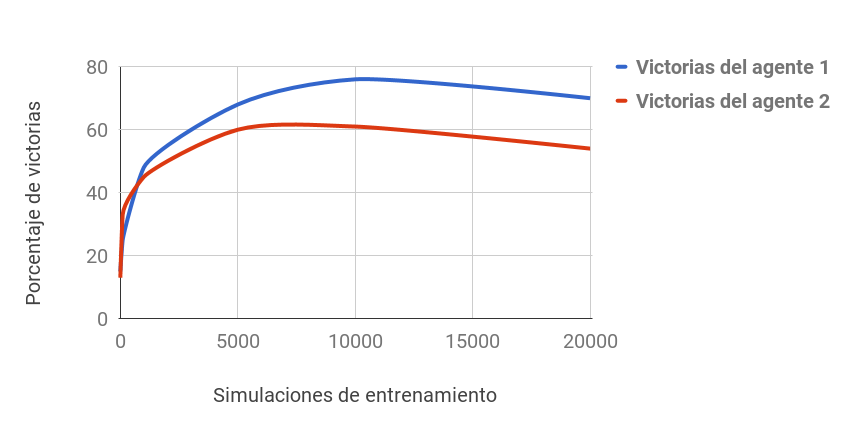
\includegraphics[width=15cm]{otros/otrasCapturas/grafico_victorias.png}}
	\caption{Porcentaje de victorias durante el entrenamiento}
	\label{graf:victorias}
\end{figure}

\begin{figure}
	\centerline{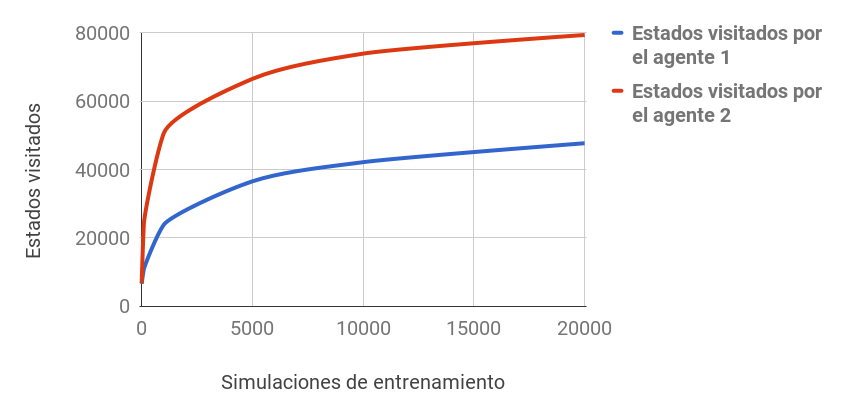
\includegraphics[width=15cm]{otros/otrasCapturas/grafico_estados.png}}
	\caption{Estados visitados durante el entrenamiento}
	\label{graf:estados}
\end{figure}

En comparación, el que llamaremos \textbf{agente 1} explicado en la sección \ref{agente1} es significativamente mejor que el \textbf{agente 2} referenciado en la sección \ref{agente2} al competir contra un personaje basado en reglas como se puede observar en la gráfica contenida en la figura \ref{graf:victorias}. Una de las razones más importantes que lleva a esto es que el agente 2, al realizar cada uno de los grupos de 100 combates para obtener las estadísticas, está peleando por primera vez contra el personaje pasado en reglas, por lo que no está tan especializado en las situaciones que se dan.

\bigskip

Por otra parte, como se puede ver en el gráfico de la figura \ref{graf:estados}, hay que tener en cuenta que el agente 2 es significativamente superior en lo que a exploración del espacio de estados se refiere. Esto genera un comportamiento mucho más completo contra jugadores humanos ya que las situaciones que los mismos crean pueden llegar a ser extremadamente raras para el agente 1. Ah haber visitado más estados se responde de forma más efectiva a oponentes con patrones poco frecuentes.

\bigskip

Algo importante que se ha observado sobre el agente 2 es que al principio de su entrenamiento, si se realizan combates contra él, su respuesta es mala comparada con la del agente 1. Esto se debe a que como entrena contra él mismo, tarda más que el agente 1 en empezar a saber que acciones son las mejores.

\bigskip

Lo que nos lleva a la \textbf{elección} del agente que se presentará en la versión final de la aplicación. Dicho agente empezará su entrenamiento contra el personaje basado en reglas para evitar ese lento comienzo que se menciona en el párrafo anterior. Luego pasará a entrenar contra él mismo para favorecer una exploración máxima de estados, el resultado es un agente con una frecuencia de victorias estimada del \textbf{80\%} y una cantidad de estados visitados de \textbf{75407}.

\bigskip

Esto favorece que la versión final presentada contenga un agente que sabe tanto responder a estados poco comunes como elegir la mejor acción en situaciones frecuentes.

\section{Observaciones}

Al analizar el comportamiento del agente elegido se han observado comportamientos relativamente complejos que no se esperaban en un principio. Algunos de los que comentaremos a continuación se pueden ver en un vídeo subido a \textit{YouTube}\footnote{disponible en: \url{https://youtu.be/NdtrxdUIRWw}}.

\bigskip

El agente suele emplear una estrategia agresiva para comenzar el combate con ventaja. Se observa como es capaz de anticiparse a cuando el enemigo estará a rango atacando primero y posicionándose en una buena situación.

\bigskip

Se considera muy interesante que cuando el enemigo escapa para evitar perder la partida, el agente no solo lo persigue sino que acorta el camino para llegar a él, realizando lo que parece una previsión de sus movimientos. Esto le sirve para atacar a donde el enemigo estará eventualmente y derrotarlo.

\bigskip

Finalmente, como se puede ver al final del vídeo referenciado, cuando el enemigo decide defenderse y el agente lo tiene a rango, espera pacientemente a que el enemigo no pueda ejecutar la acción defensiva y le asesta un ataque propio. El cual no es evitable por parte del otro personaje.

\bigskip

En general se considera que sus capacidades son destacables dada la simplicidad de las técnicas utilizadas. Incluso al desarrollador principal, muy familiarizado con su comportamiento y con el juego, es capaz de ganarle con una frecuencia aproximada del 40\%\footnote{datos obtenidos de la ejecución de 30 combates aproximadamente}.


